\documentclass[
11pt, % The default document font size, options: 10pt, 11pt, 12pt
%codirector, % Uncomment to add a codirector to the title page
]{charter} 


% El títulos de la memoria, se usa en la carátula y se puede usar el cualquier lugar del documento con el comando \ttitle
\titulo{Biofertilización de precisión} 

% Nombre del posgrado, se usa en la carátula y se puede usar el cualquier lugar del documento con el comando \degreename
%\posgrado{Carrera de Especialización en Sistemas Embebidos} 
%\posgrado{Carrera de Especialización en Internet de las Cosas} 
\posgrado{Carrera de Especialización en Inteligencia Artificial}
%\posgrado{Maestría en Sistemas Embebidos} 
%\posgrado{Maestría en Internet de las cosas}

% Tu nombre, se puede usar el cualquier lugar del documento con el comando \authorname
% IMPORTANTE: no omitir titulaciones ni tildación en los nombres, también se recomienda escribir los nombres completos (tal cual los tienen en su documento)
\autor{Lic. José Aviani}

% El nombre del director y co-director, se puede usar el cualquier lugar del documento con el comando \supname y \cosupname y \pertesupname y \pertecosupname
\director{[a definir]}
\pertenenciaDirector{[a definir]} 
\codirector{} % para que aparezca en la portada se debe descomentar la opción codirector en los parámetros de documentclass
\pertenenciaCoDirector{FIUBA}

% Nombre del cliente, quien va a aprobar los resultados del proyecto, se puede usar con el comando \clientename y \empclientename
\cliente{Ing. P.A. (MSc) Verónica Charlon}
\empresaCliente{IDICAL, INTA-CONICET}
 
\fechaINICIO{20 de octubre de 2026}		%Fecha de inicio de la cursada de GdP \fechaInicioName
\fechaFINALPlan{8 de diciembre de 2026} 	%Fecha de final de cursada de GdP
\fechaFINALTrabajo{[a definir]}	%Fecha de defensa pública del trabajo final


\begin{document}

\maketitle
\thispagestyle{empty}
\pagebreak


\thispagestyle{empty}
{\setlength{\parskip}{0pt}
\tableofcontents{}
}
\pagebreak


\section*{Registros de cambios}
\label{sec:registro}


\begin{table}[ht]
\label{tab:registro}
\centering
\begin{tabularx}{\linewidth}{@{}|c|X|c|@{}}
\hline
\rowcolor[HTML]{C0C0C0} 
Revisión & \multicolumn{1}{c|}{\cellcolor[HTML]{C0C0C0}Detalles de los cambios realizados} & Fecha      \\ \hline
0      & Creación del documento                                 &\fechaInicioName \\ \hline
%1      & Se completa hasta el punto 5 inclusive                & {día} de {mes} de 202X \\ \hline
%2      & Se completa hasta el punto 9 inclusive
%		  Se puede agregar algo más \newline
%		  En distintas líneas \newline
%		  Así                                                    & {día} de {mes} de 202X \\ \hline
%3      & Se completa hasta el punto 12 inclusive                & {día} de {mes} de 202X \\ \hline
%4      & Se completa el plan	                                 & {día} de {mes} de 202X \\ \hline

% Si hay más correcciones pasada la versión 4 también se deben especificar acá

\end{tabularx}
\end{table}

\pagebreak



\section*{Acta de constitución del proyecto}
\label{sec:acta}

\begin{flushright}
Buenos Aires, \fechaInicioName
\end{flushright}

\vspace{2cm}

Por medio de la presente se acuerda con el \authorname\hspace{1px} que su Trabajo Final de la \degreename\hspace{1px} se titulará ``\ttitle'' y consistirá en el desarrollo y evaluación de un algoritmo de regresión que integre información generada durante aplicaciones de purines con información económica asociada a fertilizantes químicos, con el objetivo de estimar la valorización económica del uso de purines como biofertilizantes.

El trabajo tendrá un presupuesto preliminar estimado de 600 horas y un costo estimado de [a definir], con fecha de inicio el \fechaInicioName\hspace{1px} y fecha de presentación pública el \fechaFinalName.

Se adjunta a esta acta la planificación inicial.

\vfill

% Esta parte se construye sola con la información que hayan cargado en el preámbulo del documento y no debe modificarla
\begin{table}[ht]
\centering
\begin{tabular}{ccc}
\begin{tabular}[c]{@{}c@{}}Dr. Ing. Ariel Lutenberg \\ Director posgrado FIUBA\end{tabular} & \hspace{2cm} & \begin{tabular}[c]{@{}c@{}}\clientename \\ \empclientename \end{tabular} \vspace{2.5cm} \\ 
\multicolumn{3}{c}{\begin{tabular}[c]{@{}c@{}} \supname \\ Director del Trabajo Final\end{tabular}} \vspace{2.5cm} \\
\end{tabular}
\end{table}





\section{1. Descripción técnica-conceptual del proyecto a realizar}
\label{sec:descripcion}

El proyecto surge de una propuesta del Instituto de Investigación de la Cadena Láctea (IDICAL, INTA-CONICET), en articulación con las empresas Loma Fértil y Agronorte. El tema fue seleccionado entre las propuestas de Trabajo Final ofrecidas a los alumnos de la Carrera de Especialización en Inteligencia Artificial.

En las explotaciones pecuarias, los purines constituyen una fuente de nutrientes que puede aprovecharse como biofertilizante y reducir la necesidad de utilizar fertilizantes químicos. Sin embargo, su composición presenta una importante variabilidad. Mediante los métodos tradicionales de aplicación se conoce, en general, el volumen distribuido, pero no la cantidad efectiva de nutrientes incorporados al suelo. Esto dificulta tanto una dosificación adecuada como la valoración económica de su aprovechamiento.

Actualmente, el sistema HarvestLab 3000, mediante la tecnología \textit{Manure Sensing} y el uso de espectroscopía de infrarrojo cercano (\textit{Near-Infrared Spectroscopy}, NIRS), permite analizar el purín durante su aplicación. El sistema obtiene mediciones en tiempo real de su composición nutricional y genera información georreferenciada de los nutrientes aplicados en cada lote. Como parte de los trabajos desarrollados por INTA, Loma Fértil y Agronorte, se realizan tareas de validación regional mediante la comparación de las lecturas del sensor con análisis de laboratorio.

Esta tecnología permite conocer con mayor precisión qué nutrientes se aplican, pero la información obtenida no se traduce directamente en una estimación de su valor económico. El problema que aborda este Trabajo Final consiste en aprovechar los datos generados durante las aplicaciones para estimar económicamente el uso del purín como biofertilizante y compararlo con alternativas de fertilización convencional.

La solución propuesta consiste en desarrollar y evaluar un algoritmo de regresión que integre los datos obtenidos mediante HarvestLab 3000 con variables operativas e información económica de fertilizantes químicos. La información disponible contempla concentraciones de nutrientes —entre ellos nitrógeno, fósforo y potasio—, dosis aplicadas, tiempos operativos, distancias y datos georreferenciados. Además, se incorporarán precios actualizados de fertilizantes.

Uno de los desafíos iniciales del proyecto será acceder a los datos necesarios para el desarrollo del modelo. La información generada por HarvestLab 3000 se encuentra almacenada en la plataforma de John Deere, por lo que será necesario gestionar su acceso y determinar la forma adecuada de extraerla para su posterior procesamiento y análisis. La disponibilidad, estructura y calidad de estos datos condicionarán las etapas posteriores del proyecto.

La variable objetivo definitiva se establecerá durante la etapa inicial del proyecto junto con INTA, Loma Fértil y Agronorte. Entre las alternativas consideradas se encuentran el valor económico por hectárea, el ahorro respecto de una estrategia de fertilización convencional, una medida de costo/beneficio de la aplicación u otra variable económica derivada de las mediciones disponibles y de la información de mercado.

La propuesta de valor radica en transformar mediciones agronómicas obtenidas durante las aplicaciones en información económica cuantificable. Los usuarios directos de la solución serán Loma Fértil y sus técnicos, quienes podrán disponer de información adicional para evaluar los beneficios económicos del uso de purines frente a alternativas de fertilización convencional. La integración de datos reales y georreferenciados con información económica actualizada y técnicas de aprendizaje automático constituye el aspecto central de la solución propuesta.

En la figura 1 se presenta el diagrama en bloques de la solución. Se observan dos fuentes principales de información: los datos generados por HarvestLab 3000 y la información económica asociada a fertilizantes. Los datos serán obtenidos, integrados y acondicionados antes de utilizarse para desarrollar el algoritmo de regresión. Posteriormente, se evaluará y validará el modelo obtenido. Como resultado se espera generar una estimación económica por unidad de superficie que pueda utilizarse como información de apoyo para la toma de decisiones.

\begin{figure}[htpb]
\centering 
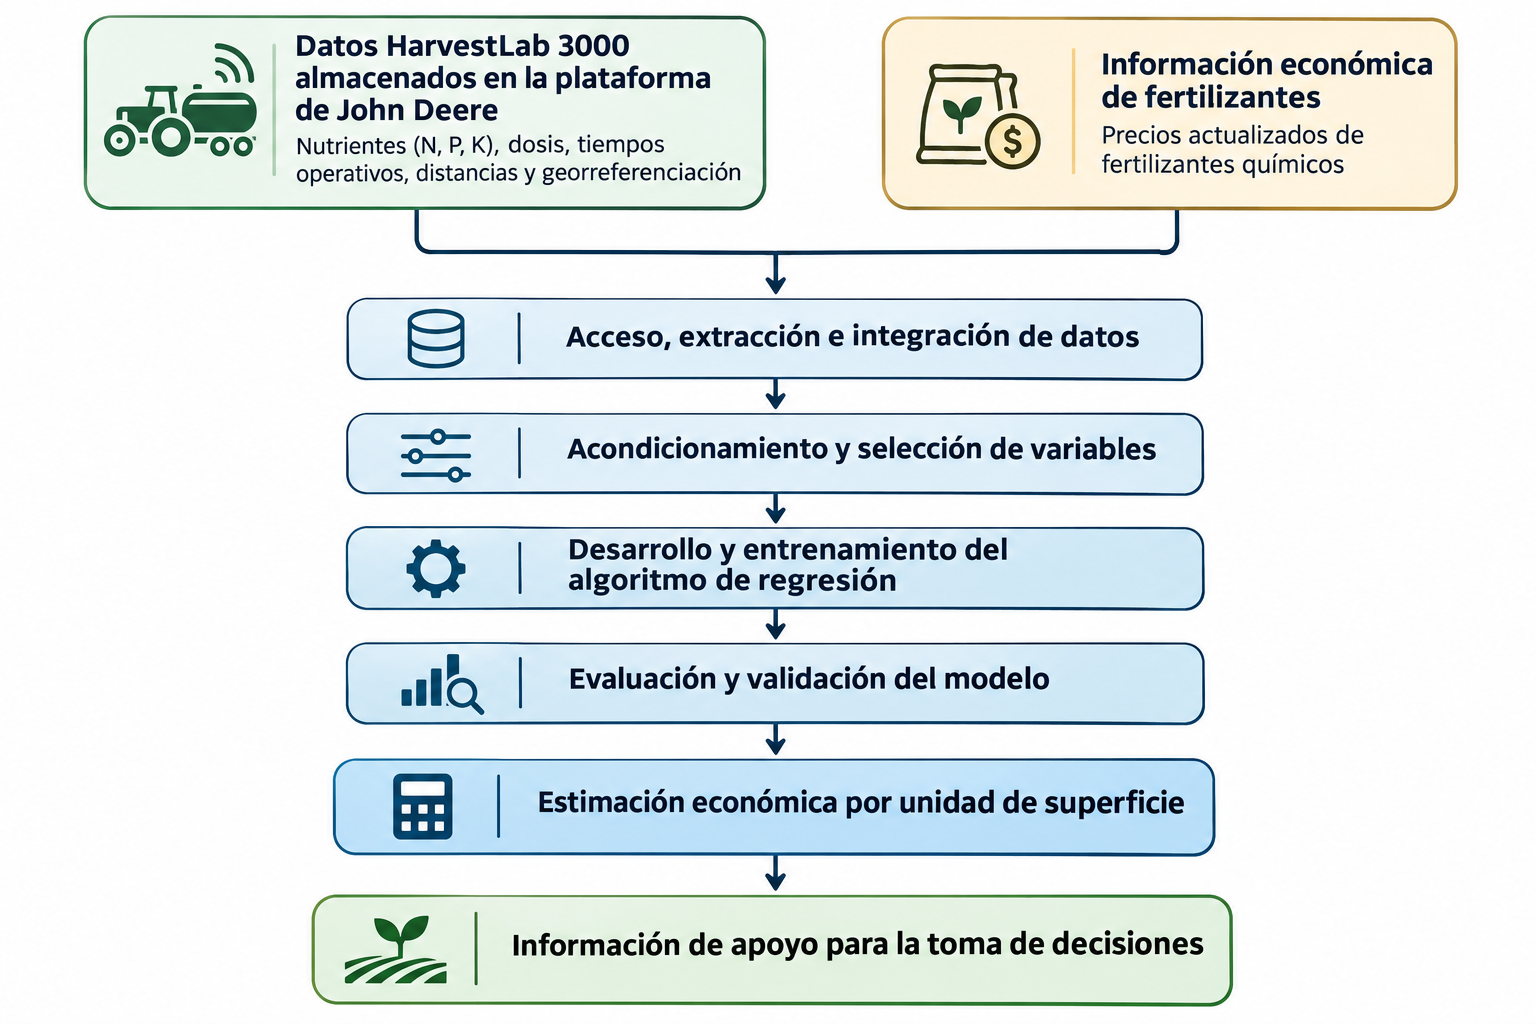
\includegraphics[width=.65\textwidth]{./Figuras/01_Flujo_datos_agricolas_y_decisiones.png}
\caption{Flujo de datos agrícolas y decisiones.}
\label{fig:diagBloques}
\end{figure}





\section{2. Identificación y análisis de los interesados}
\label{sec:interesados}

Los principales interesados identificados para el proyecto se presentan en la siguiente tabla.

\begin{table}[ht]
%\caption{Identificación de los interesados}
%\label{tab:interesados}
\begin{tabularx}{\linewidth}{@{}|l|X|X|l|@{}}
\hline
\rowcolor[HTML]{C0C0C0} 
Rol & Nombre y Apellido & Organización & Puesto \\ \hline
Cliente & \clientename & \empclientename & Investigadora y referente del proyecto \\ \hline
Responsable & \authorname & FIUBA & Alumno \\ \hline
Colaborador & Luis Hermoso & Loma Fértil & Responsable de Loma Fértil \\ \hline
Colaborador & Alejandro Regalini & Agronorte & Representante de Agronorte \\ \hline
Colaborador & Emmanuel Rista & Agronorte & Referente para el acceso a los datos \\ \hline
Orientador & \supname & \pertesupname & Director del Trabajo Final \\ \hline
Usuario final & Loma Fértil y sus técnicos & Loma Fértil & - \\ \hline
\end{tabularx}
\end{table}

\textbf{Cliente}: Verónica Charlon será la principal referente del proyecto y participará en la definición de los objetivos, las variables de interés y los criterios de evaluación de los resultados. Además, actuará como interlocutora entre las distintas organizaciones involucradas y promoverá el desarrollo del proyecto.

\textbf{Responsable}: José Aviani será responsable de la planificación y ejecución del proyecto, del procesamiento y análisis de los datos, del desarrollo y validación del modelo de regresión y de la elaboración de los entregables correspondientes al Trabajo Final.

\textbf{Colaboradores}: Luis Hermoso y Alejandro Regalini aportarán conocimiento del dominio, de las aplicaciones realizadas y del contexto productivo en el que se utiliza la tecnología. Emmanuel Rista colaborará específicamente en la gestión del acceso a los datos generados por HarvestLab 3000 y almacenados en la plataforma de John Deere.

\textbf{Orientador}: el director del Trabajo Final está por definir. Su función será orientar el desarrollo académico y técnico del proyecto y supervisar el cumplimiento de los objetivos establecidos.

\textbf{Usuario final}: Loma Fértil y sus técnicos constituyen los usuarios directos de los resultados del proyecto. Se espera que la información económica obtenida a partir del modelo contribuya a evaluar las aplicaciones de purines y facilite la toma de decisiones asociadas a su utilización como biofertilizantes.





\section{3. Propósito del proyecto}
\label{sec:proposito}

Proporcionar a Loma Fértil y a sus técnicos una herramienta que permita transformar los datos generados por HarvestLab 3000 en información económica útil para cuantificar el valor de las aplicaciones de purines y mejorar la toma de decisiones. Como propósito complementario, se busca favorecer un aprovechamiento más eficiente de los nutrientes presentes en los purines y reducir la dependencia de fertilizantes químicos mediante una mejor valoración de su uso como biofertilizantes.





\section{4. Alcance del proyecto}
\label{sec:alcance}

El proyecto incluye:

\begin{itemize}
\item La gestión del acceso y la extracción de los datos generados por HarvestLab 3000 y almacenados en la plataforma de John Deere.
\item El análisis exploratorio y acondicionamiento del conjunto de datos, incluyendo limpieza, tratamiento de valores faltantes o anómalos, transformación y selección de variables.
\item La definición, junto con INTA, Loma Fértil y Agronorte, de la variable económica objetivo que se utilizará para el desarrollo del modelo.
\item La obtención y preparación de información de precios de fertilizantes químicos necesaria para la valorización económica de las aplicaciones.
\item La evaluación y comparación de distintas alternativas de regresión para seleccionar la más adecuada para el problema planteado.
\item El desarrollo, entrenamiento, evaluación y validación del algoritmo de regresión seleccionado.
\item El análisis de la relevancia de las variables utilizadas en las estimaciones.
\item El desarrollo de un prototipo básico que permita utilizar el modelo obtenido y visualizar sus resultados mediante una interfaz de usuario sencilla.
\item La documentación de la solución desarrollada y de los resultados obtenidos.
\end{itemize}

El presente proyecto no incluye:

\begin{itemize}
\item La integración automática del modelo con HarvestLab 3000, la plataforma de John Deere ni los sistemas informáticos de Loma Fértil.
\item La consulta automática de precios de fertilizantes a fuentes externas.
\item La calibración regional del sensor HarvestLab 3000 ni la validación de sus mediciones mediante análisis de laboratorio.
\item El desarrollo de la segunda línea planteada en la propuesta original (propuesta de Trabajo Final ofrecida a los alumnos de la Carrera de Especialización en Inteligencia Artificial), correspondiente a la combinación de datos de HarvestLab 3000 —N, P, K y materia seca— con variables externas, como tipo de suelo, humedad, temperatura y pronóstico climático, para predecir el riesgo de lixiviación, las emisiones de óxido nitroso y el impacto sobre la huella de carbono.
\item La validación del modelo para regiones, establecimientos, tipos de purines o condiciones productivas diferentes de las representadas en el conjunto de datos disponible para el proyecto.
\item El desarrollo de una aplicación productiva o de una interfaz de usuario de complejidad superior al prototipo básico previsto.
\end{itemize}





\section{5. Supuestos del proyecto}
\label{sec:supuestos}

Para el desarrollo del presente proyecto se supone que:

\begin{itemize}
\item Se obtendrá acceso a la plataforma de John Deere y a los datos necesarios para el desarrollo del proyecto.
\item El conjunto de datos disponible tendrá cantidad, variedad y calidad suficientes para entrenar y validar el modelo de regresión.
\item Los datos extraídos podrán transformarse a un formato adecuado para su procesamiento y análisis, independientemente del formato original en que se encuentren almacenados.
\item Se dispondrá de fuentes públicas y confiables con información de precios de fertilizantes suficiente para construir las variables económicas necesarias.
\item Los principales interesados —Verónica Charlon, Luis Hermoso, Alejandro Regalini y Emmanuel Rista— estarán disponibles para resolver consultas de dominio, colaborar en la definición de la variable objetivo y facilitar el acceso a la información requerida.
\item Se contará con los recursos de cómputo y las herramientas necesarias para realizar el procesamiento de datos, el entrenamiento, la evaluación y la validación del modelo.
\item Existe un acuerdo previo de uso de los datos para fines académicos en el marco del Trabajo Final. Por lo tanto, se supone que no existirán impedimentos relacionados con la autorización para utilizar la información necesaria durante el desarrollo del proyecto.
\end{itemize}





\section{6. Product Backlog}
\label{sec:backlog}

El \textit{Product Backlog} se organiza en cuatro épicas que representan los principales bloques funcionales del proyecto. Para cada historia de usuario se indica su prioridad, obligatoriedad y ponderación en \textit{Story Points}.

Para estimar los \textit{Story Points} se consideran tres dimensiones: \textbf{dificultad}, asociada a la cantidad de trabajo; \textbf{complejidad}, vinculada con el nivel técnico; e \textbf{incertidumbre}, relacionada con el riesgo, la novedad o la experiencia previa. Para cada dimensión se utiliza la siguiente escala: baja = 1, media = 3 y alta = 5. Los valores se suman y, cuando el resultado no pertenece a la serie de Fibonacci, se redondea hacia el valor superior más próximo.

La estimación global del proyecto es de \textbf{600 horas}. Los \textit{Story Points} se utilizan como medida relativa entre historias de usuario y no representan una conversión directa a horas.

\begin{itemize}

  \item \textbf{\'{E}pica 1 - Acceso y preparación de los datos}
    \begin{itemize}

      \item \textbf{HU1} Como \textbf{científico de datos}, quiero acceder y extraer los datos generados por HarvestLab 3000 y almacenados en la plataforma de John Deere para disponer de la información necesaria para el desarrollo del modelo.
        \begin{itemize}
          \item Prioridad: Alta.
          \item Obligatoriedad: Obligatoria.
          \item Dificultad: Media (3).
          \item Complejidad: Media (3).
          \item Incertidumbre: Alta (5).
          \item Suma: 11.
          \item \textit{Story Points}: \textbf{13}.
        \end{itemize}

      \item \textbf{HU2} Como \textbf{científico de datos}, quiero acondicionar y transformar los datos extraídos para obtener un conjunto de datos consistente y adecuado para su análisis y modelado.
        \begin{itemize}
          \item Prioridad: Alta.
          \item Obligatoriedad: Obligatoria.
          \item Dificultad: Alta (5).
          \item Complejidad: Media (3).
          \item Incertidumbre: Alta (5).
          \item Suma: 13.
          \item \textit{Story Points}: \textbf{13}.
        \end{itemize}

    \end{itemize}


  \item \textbf{\'{E}pica 2 - Construcción de la estimación económica}
    \begin{itemize}

      \item \textbf{HU3} Como \textbf{científico de datos}, quiero integrar los datos de las aplicaciones con información de precios de fertilizantes para construir las variables económicas necesarias para el modelo.
        \begin{itemize}
          \item Prioridad: Alta.
          \item Obligatoriedad: Obligatoria.
          \item Dificultad: Media (3).
          \item Complejidad: Media (3).
          \item Incertidumbre: Baja (1).
          \item Suma: 7.
          \item \textit{Story Points}: \textbf{8}.
        \end{itemize}

      \item \textbf{HU4} Como \textbf{usuario final}, quiero obtener una estimación económica por unidad de superficie a partir de los datos de una aplicación para evaluar el valor económico del uso del purín como biofertilizante.
        \begin{itemize}
          \item Prioridad: Alta.
          \item Obligatoriedad: Obligatoria.
          \item Dificultad: Alta (5).
          \item Complejidad: Alta (5).
          \item Incertidumbre: Media (3).
          \item Suma: 13.
          \item \textit{Story Points}: \textbf{13}.
        \end{itemize}

    \end{itemize}


  \item \textbf{\'{E}pica 3 - Modelado, evaluación y validación}
    \begin{itemize}

      \item \textbf{HU5} Como \textbf{científico de datos}, quiero evaluar distintas alternativas de regresión para seleccionar el modelo que presente el desempeño más adecuado para el problema planteado.
        \begin{itemize}
          \item Prioridad: Alta.
          \item Obligatoriedad: Obligatoria.
          \item Dificultad: Alta (5).
          \item Complejidad: Alta (5).
          \item Incertidumbre: Alta (5).
          \item Suma: 15.
          \item \textit{Story Points}: \textbf{21}.
        \end{itemize}

      \item \textbf{HU6} Como \textbf{usuario final}, quiero disponer de información sobre el desempeño del modelo y sobre las variables relevantes de la estimación para interpretar adecuadamente los resultados obtenidos.
        \begin{itemize}
          \item Prioridad: Media.
          \item Obligatoriedad: Obligatoria.
          \item Dificultad: Media (3).
          \item Complejidad: Media (3).
          \item Incertidumbre: Baja (1).
          \item Suma: 7.
          \item \textit{Story Points}: \textbf{8}.
        \end{itemize}

    \end{itemize}


  \item \textbf{\'{E}pica 4 - Prototipo y presentación de resultados}
    \begin{itemize}

      \item \textbf{HU7} Como \textbf{desarrollador}, quiero implementar un prototipo con una interfaz básica que permita seleccionar datos previamente cargados y ejecutar el modelo para facilitar su utilización por los usuarios de Loma Fértil.
        \begin{itemize}
          \item Prioridad: Alta.
          \item Obligatoriedad: Obligatoria.
          \item Dificultad: Alta (5).
          \item Complejidad: Media (3).
          \item Incertidumbre: Media (3).
          \item Suma: 11.
          \item \textit{Story Points}: \textbf{13}.
        \end{itemize}

      La modalidad exacta de selección de los datos previamente cargados se definirá durante el desarrollo del proyecto.

      \item \textbf{HU8} Como \textbf{usuario final}, quiero visualizar la estimación económica junto con información complementaria y disponer de una opción de exportación para analizar y conservar los resultados obtenidos.
        \begin{itemize}
          \item Prioridad: Media.
          \item Obligatoriedad: Obligatoria.
          \item Dificultad: Media (3).
          \item Complejidad: Media (3).
          \item Incertidumbre: Media (3).
          \item Suma: 9.
          \item \textit{Story Points}: \textbf{13}.
        \end{itemize}

      La información complementaria a visualizar se definirá durante el desarrollo del proyecto. Entre las alternativas consideradas se encuentran los nutrientes aplicados, su valor equivalente en fertilizantes y comparaciones con alternativas de fertilización convencional. Asimismo, se evaluarán posibles formatos de exportación, como CSV o PDF, sin definir en esta etapa un formato obligatorio.

    \end{itemize}

\end{itemize}





\section{7. Criterios de aceptación de historias de usuario}
\label{sec:criteriosAceptacion}

Los criterios de aceptación permiten determinar de manera objetiva cuándo cada historia de usuario puede considerarse completada. Se definen a continuación criterios funcionales, técnicos y, cuando corresponde, de presentación de resultados.

\begin{itemize}

  \item \textbf{\'{E}pica 1 - Acceso y preparación de los datos}
    \begin{itemize}

      \item \textbf{Criterios de aceptación HU1}
        \begin{itemize}
          \item Se obtiene acceso efectivo a los datos generados por HarvestLab 3000 y almacenados en la plataforma de John Deere.
          \item Los datos necesarios para el desarrollo pueden extraerse desde la fuente disponible y almacenarse para su posterior procesamiento.
          \item El procedimiento utilizado para acceder y extraer los datos queda documentado de manera que pueda repetirse durante el desarrollo del proyecto.
        \end{itemize}

      \item \textbf{Criterios de aceptación HU2}
        \begin{itemize}
          \item Los datos extraídos pueden transformarse a un formato adecuado para su procesamiento y análisis.
          \item Se identifican y tratan los valores faltantes, anómalos o inconsistentes mediante criterios documentados.
          \item El conjunto de datos acondicionado puede cargarse y procesarse sin errores que impidan su utilización en las etapas posteriores.
          \item Se conservan las variables consideradas relevantes para el análisis y desarrollo del modelo.
        \end{itemize}

    \end{itemize}


  \item \textbf{\'{E}pica 2 - Construcción de la estimación económica}
    \begin{itemize}

      \item \textbf{Criterios de aceptación HU3}
        \begin{itemize}
          \item Se incorpora información de precios de fertilizantes proveniente de al menos una fuente pública y confiable.
          \item Se documentan la fuente y la fecha de referencia de la información económica utilizada.
          \item Se construyen las variables económicas necesarias para relacionar la información de las aplicaciones con los precios de fertilizantes.
          \item El procedimiento utilizado para construir las variables económicas queda documentado y puede reproducirse a partir de los mismos datos de entrada.
        \end{itemize}

      \item \textbf{Criterios de aceptación HU4}
        \begin{itemize}
          \item A partir de los datos correspondientes a una aplicación, el sistema genera una estimación económica expresada por unidad de superficie.
          \item La estimación se calcula utilizando la variable objetivo acordada con los interesados y las variables definidas durante el desarrollo del modelo.
          \item Ante los mismos datos de entrada y la misma versión del modelo, se obtiene el mismo resultado de la estimación.
          \item El resultado se presenta identificando la variable estimada, el valor obtenido y la unidad de medida correspondiente.
        \end{itemize}

    \end{itemize}


  \item \textbf{\'{E}pica 3 - Modelado, evaluación y validación}
    \begin{itemize}

      \item \textbf{Criterios de aceptación HU5}
        \begin{itemize}
          \item Se desarrollan y evalúan al menos tres alternativas de regresión.
          \item Todas las alternativas se evalúan utilizando el mismo esquema de preparación de datos, partición o validación y las mismas métricas definidas para la comparación.
          \item Las métricas de evaluación se establecen durante el desarrollo en función de las características del problema y de la variable objetivo.
          \item La selección del modelo final se justifica mediante la comparación de los resultados obtenidos y queda documentada.
        \end{itemize}

      \item \textbf{Criterios de aceptación HU6}
        \begin{itemize}
          \item Se presentan las métricas utilizadas para evaluar el desempeño del modelo seleccionado.
          \item Se identifican y presentan las variables que muestran mayor relevancia para las estimaciones mediante una técnica adecuada al modelo utilizado.
          \item La información sobre desempeño y relevancia de variables se presenta mediante valores, tablas o gráficos identificados y acompañados por una descripción de su significado.
          \item Se documentan las principales limitaciones del modelo que deban considerarse al interpretar los resultados.
        \end{itemize}

    \end{itemize}


  \item \textbf{\'{E}pica 4 - Prototipo y presentación de resultados}
    \begin{itemize}

      \item \textbf{Criterios de aceptación HU7}
        \begin{itemize}
          \item El prototipo permite seleccionar un conjunto de datos previamente cargado sin necesidad de modificar el código fuente.
          \item El usuario puede ejecutar el modelo sobre los datos seleccionados desde la interfaz del prototipo.
          \item Una vez ejecutado el modelo, el prototipo presenta la estimación económica obtenida.
          \item La interfaz identifica de manera clara el conjunto de datos seleccionado, la acción necesaria para ejecutar el modelo y el resultado generado.
        \end{itemize}

      La modalidad específica mediante la cual se realizará la selección de los datos previamente cargados se definirá durante el desarrollo del proyecto.

      \item \textbf{Criterios de aceptación HU8}
        \begin{itemize}
          \item La interfaz muestra la estimación económica obtenida y al menos un tipo de información complementaria asociada al resultado.
          \item La interfaz muestra al menos un tipo de información complementaria acordado durante la ejecución del proyecto.
          \item Los resultados se presentan con descripciones y unidades que permitan interpretar correctamente la información mostrada.
          \item El prototipo permite exportar los resultados en al menos un formato definido durante el desarrollo del proyecto.
          \item El archivo exportado contiene, como mínimo, la estimación económica y la información complementaria presentada por el prototipo.
        \end{itemize}

      El formato específico de exportación se definirá durante el desarrollo del proyecto. Entre las alternativas consideradas se encuentran CSV y PDF.

    \end{itemize}

\end{itemize}





\section{8. Fases de CRISP-DM}

Para el desarrollo del proyecto se utilizará la metodología CRISP-DM (\textit{Cross-Industry Standard Process for Data Mining}) como marco de referencia para organizar las actividades relacionadas con la comprensión del problema, el tratamiento de los datos, el desarrollo del modelo y su evaluación. Las decisiones específicas correspondientes a cada fase se ajustarán durante la ejecución del proyecto en función de la disponibilidad, estructura y características de los datos obtenidos.

\begin{enumerate}

  \item \textbf{Comprensión del negocio}

  El objetivo del proyecto es transformar los datos generados durante las aplicaciones de purines en información económica que permita cuantificar su valor como biofertilizante por unidad de superficie y facilite la toma de decisiones de Loma Fértil y sus técnicos.

  El valor agregado de la aplicación de técnicas de inteligencia artificial consiste en desarrollar un modelo capaz de relacionar las variables disponibles en los datos de las aplicaciones con información económica asociada a fertilizantes y generar una estimación a partir de dicha relación.

  Como criterios generales de éxito se considerará la obtención de una estimación económica interpretable por los usuarios, el desarrollo de un modelo evaluado y validado mediante métricas adecuadas y la disponibilidad de un prototipo básico que permita consultar los resultados. Las métricas y condiciones específicas de éxito se definirán y ajustarán durante la ejecución del proyecto junto con los interesados.


  \item \textbf{Comprensión de los datos}

  Los datos principales provendrán del sistema HarvestLab 3000 y se encuentran almacenados en la plataforma de John Deere. La información disponible contempla variables relacionadas con la composición de los purines y con las aplicaciones realizadas, entre ellas concentraciones de nitrógeno, fósforo y potasio, dosis aplicadas, tiempos operativos, distancias y datos georreferenciados.

  Además, se utilizará información económica proveniente de fuentes públicas y confiables, principalmente precios de fertilizantes químicos, para construir las variables necesarias para la valorización económica.

  Durante esta fase se analizarán la estructura, cantidad, calidad, consistencia y representatividad de los datos disponibles. La cantidad efectiva de registros, su formato y el nivel de detalle se determinarán una vez obtenido el acceso a la información de la plataforma de John Deere.


  \item \textbf{Preparación de los datos}

  Los datos obtenidos serán acondicionados para su utilización en las etapas de análisis y modelado. Esta fase incluirá la transformación de los datos extraídos a un formato adecuado para su procesamiento, independientemente de su formato original.

  Se realizará la identificación y tratamiento de valores faltantes, anómalos o inconsistentes. También se evaluarán transformaciones, normalizaciones y mecanismos de selección o generación de variables que resulten necesarios para el desarrollo del modelo.

  Entre las características inicialmente consideradas se encuentran las concentraciones de nutrientes, dosis aplicadas, variables operativas y georreferenciadas, junto con las variables económicas construidas a partir de los precios de fertilizantes. La selección definitiva de características y las transformaciones a aplicar se establecerán durante la ejecución del proyecto a partir del análisis exploratorio de los datos.


  \item \textbf{Modelado}

  El problema se abordará como un problema de regresión orientado a estimar una variable económica por unidad de superficie. La variable objetivo definitiva será acordada durante la ejecución del proyecto junto con INTA, Loma Fértil y Agronorte.

  Se evaluarán distintas alternativas de regresión. Entre las opciones inicialmente consideradas se encuentran modelos de regresión lineal y variantes regularizadas, árboles de decisión, métodos de ensamble, \textit{Random Forest} y \textit{Gradient Boosting}. Estas alternativas son preliminares y podrán modificarse o ampliarse en función de las características del conjunto de datos.

  Durante esta fase se desarrollarán, entrenarán y ajustarán al menos tres alternativas de regresión. La selección del modelo final se realizará a partir de la comparación de sus resultados y de las métricas definidas durante la ejecución del proyecto.


  \item \textbf{Evaluación del modelo}

  Los modelos desarrollados serán evaluados mediante métricas adecuadas para problemas de regresión. Entre las métricas inicialmente consideradas se encuentran el error absoluto medio (MAE, del inglés \textit{Mean Absolute Error}), la raíz del error cuadrático medio (RMSE, del inglés \textit{Root Mean Squared Error}) y el coeficiente de determinación \(R^2\). La selección definitiva de las métricas se realizará durante la ejecución del proyecto en función de la variable objetivo y de las características de los datos.

  Se utilizará una estrategia de separación entre datos de entrenamiento y evaluación. Si la cantidad y las características de los datos lo permiten, se considerará además el uso de técnicas de validación cruzada. La estrategia específica de validación se definirá luego de la etapa de comprensión y análisis exploratorio de los datos.

  La evaluación no se limitará al desempeño predictivo. También se analizará la relevancia de las variables utilizadas, las limitaciones del modelo y la consistencia de los resultados respecto de los objetivos definidos para el proyecto.


  \item \textbf{Despliegue del modelo}

  En el contexto de este proyecto, el despliegue consistirá en integrar el modelo seleccionado en un prototipo básico con una interfaz sencilla que permita utilizar datos previamente cargados y visualizar los resultados obtenidos.

  El prototipo deberá permitir ejecutar el modelo, consultar la estimación económica y acceder a información complementaria asociada al resultado. También se prevé incorporar al menos una opción de exportación. La modalidad de selección de datos, la información adicional a presentar, el formato de exportación y las herramientas concretas para implementar el prototipo se definirán durante la ejecución del proyecto.

  Esta fase no contempla un despliegue productivo ni la integración automática con HarvestLab 3000, la plataforma de John Deere o los sistemas informáticos de Loma Fértil.

\end{enumerate}





\section{9. Desglose del trabajo en tareas}
\label{sec:wbs}

A partir de las historias de usuario definidas en la sección 6, se propone el siguiente desglose preliminar en tareas técnicas. Las estimaciones horarias y las decisiones relacionadas con herramientas, mecanismos de acceso a los datos, técnicas de procesamiento, algoritmos y tecnologías de implementación podrán ajustarse durante la ejecución del proyecto a medida que se disponga de mayor información.

\begin{itemize}

  \item \textbf{\'{E}pica 1 - Acceso y preparación de los datos}

  \begin{center}
  \begin{tabular}{|c|p{9cm}|c|c|}
  \hline
  \textbf{HU} & \textbf{Tarea técnica} & \textbf{Estimación} & \textbf{Prioridad} \\
  \hline
  HU1 & Relevar y verificar el mecanismo disponible para acceder a los datos almacenados en la plataforma de John Deere. & 4 h & Alta \\
  \hline
  HU1 & Realizar una extracción inicial de datos y almacenarla para su posterior procesamiento. & 6 h & Alta \\
  \hline
  HU1 & Verificar la integridad, legibilidad y posibilidad de procesamiento de los datos extraídos, y documentar el procedimiento utilizado. & 4 h & Alta \\
  \hline
  HU2 & Realizar un perfilado inicial del conjunto de datos para identificar tipos de variables, valores faltantes, anomalías e inconsistencias. & 6 h & Alta \\
  \hline
  HU2 & Implementar las transformaciones y procedimientos de limpieza necesarios para obtener un conjunto de datos adecuado para el modelado. & 8 h & Alta \\
  \hline
  HU2 & Verificar la reproducibilidad del acondicionamiento y la conservación de las variables consideradas relevantes para el análisis. & 5 h & Alta \\
  \hline
  \end{tabular}
  \end{center}

  El mecanismo específico de acceso y extracción, así como las transformaciones concretas necesarias, se definirán durante la ejecución del proyecto luego de analizar la estructura real de los datos disponibles.


  \item \textbf{\'{E}pica 2 - Construcción de la estimación económica}

  \begin{center}
  \begin{tabular}{|c|p{9cm}|c|c|}
  \hline
  \textbf{HU} & \textbf{Tarea técnica} & \textbf{Estimación} & \textbf{Prioridad} \\
  \hline
  HU3 & Identificar una o más fuentes públicas y confiables de precios de fertilizantes y registrar su información de referencia. & 4 h & Alta \\
  \hline
  HU3 & Implementar el procedimiento de transformación e integración necesario para construir las variables económicas a partir de los datos de aplicaciones y precios de fertilizantes. & 6 h & Alta \\
  \hline
  HU4 & Definir la estructura de entradas y salidas necesaria para generar la estimación económica por unidad de superficie a partir de la variable objetivo acordada. & 4 h & Alta \\
  \hline
  HU4 & Implementar y verificar el procedimiento que genere la estimación económica para los datos correspondientes a una aplicación. & 6 h & Alta \\
  \hline
  \end{tabular}
  \end{center}

  La fuente definitiva de precios, la variable económica objetivo y las transformaciones utilizadas para construir las variables económicas se definirán durante la ejecución del proyecto junto con los interesados.


  \item \textbf{\'{E}pica 3 - Modelado, evaluación y validación}

  \begin{center}
  \begin{tabular}{|c|p{9cm}|c|c|}
  \hline
  \textbf{HU} & \textbf{Tarea técnica} & \textbf{Estimación} & \textbf{Prioridad} \\
  \hline
  HU5 & Definir el protocolo preliminar de comparación de modelos, incluyendo alternativas de regresión, partición de datos y métricas de evaluación. & 4 h & Alta \\
  \hline
  HU5 & Implementar y ejecutar el entrenamiento de al menos tres alternativas de regresión utilizando un esquema común de preparación y evaluación. & 8 h & Alta \\
  \hline
  HU5 & Comparar los resultados obtenidos, seleccionar el modelo más adecuado y documentar los criterios utilizados para la selección. & 6 h & Alta \\
  \hline
  HU6 & Calcular y organizar las métricas de desempeño correspondientes al modelo seleccionado. & 4 h & Media \\
  \hline
  HU6 & Analizar la relevancia de las variables y documentar las principales limitaciones que deban considerarse para interpretar las estimaciones. & 6 h & Media \\
  \hline
  \end{tabular}
  \end{center}

  Los algoritmos concretos, las métricas, la estrategia de validación y las técnicas utilizadas para analizar la relevancia de las variables se definirán y ajustarán durante la ejecución del proyecto en función de las características de los datos y del modelo desarrollado.


  \item \textbf{\'{E}pica 4 - Prototipo y presentación de resultados}

  \begin{center}
  \begin{tabular}{|c|p{9cm}|c|c|}
  \hline
  \textbf{HU} & \textbf{Tarea técnica} & \textbf{Estimación} & \textbf{Prioridad} \\
  \hline
  HU7 & Definir el flujo básico de interacción del prototipo y el mecanismo preliminar para seleccionar conjuntos de datos previamente cargados. & 4 h & Alta \\
  \hline
  HU7 & Implementar una interfaz básica que permita seleccionar los datos y ejecutar el modelo sin modificar el código fuente. & 8 h & Alta \\
  \hline
  HU7 & Verificar el funcionamiento de extremo a extremo del prototipo y la presentación de la estimación económica obtenida. & 5 h & Alta \\
  \hline
  HU8 & Definir, junto con los interesados, la información complementaria a visualizar y al menos un formato de exportación. & 3 h & Media \\
  \hline
  HU8 & Implementar la visualización de la estimación económica y de al menos un tipo de información complementaria. & 6 h & Media \\
  \hline
  HU8 & Implementar la exportación de los resultados y verificar que el archivo generado contenga la información requerida. & 5 h & Media \\
  \hline
  \end{tabular}
  \end{center}

  La tecnología de implementación del prototipo, el mecanismo definitivo de selección de datos, la información complementaria presentada y el formato de exportación se definirán durante la ejecución del proyecto.

\end{itemize}

Las tareas detalladas en esta sección representan las actividades técnicas directamente asociadas a las historias de usuario seleccionadas y totalizan \textbf{112 horas estimadas}. Este valor no representa la duración total del proyecto, estimada en \textbf{600 horas}, ya que no incluye la totalidad de las actividades de planificación, investigación, iteración, reuniones, documentación, redacción de la memoria, revisión y preparación de la defensa.





% JA: Completar los "[a definir]" y otros "definir".
% JA: Hasta acá completo.







\section{10. Planificación de Sprints}

Organizar las tareas técnicas del proyecto en sprints de trabajo que permitan distribuir de forma equilibrada la carga horaria total, estimada en 600 horas.

\textbf{Consigna:}
\begin{itemize}
  \item Completar una tabla que relacione sprints con HU y tareas técnicas correspondientes.
  \item Incluir estimación en horas para cada tarea.
  \item Indicar responsable y porcentaje de avance estimado o completado.
  \item Contemplar también tareas de planificación, documentación, redacción de memoria y preparación de defensa.
\end{itemize}

\textbf{Conceptos clave:}
\begin{itemize}
  \item Una \'{e}pica es una unidad funcional amplia; una historia de usuario es una funcionalidad concreta; un sprint es una unidad de tiempo donde se ejecutan tareas.
  \item Las tareas son el nivel más desagregado: permiten estimar tiempos, asignar responsables y monitorear progreso.
\end{itemize}

\textbf{Duración sugerida:}
\begin{itemize}
  \item Para un proyecto de 600 h, se recomienda planificar entre 10 y 12 sprints de aproximadamente 2 semanas cada uno.
  \item Asignar entre 45 y 50 horas efectivas por sprint a tareas técnicas.
  \item Reservar 100 a 120 h para actividades no técnicas (planificación, escritura, reuniones, defensa).
\end{itemize}

\textbf{Importante:}
\begin{itemize}
  \item En proyectos individuales, el responsable suele ser el propio autor.
  \item Aun así, desagregar tareas facilita el seguimiento y mejora continua.
\end{itemize}

\textbf{Conversión opcional de Story Points a horas:}
\begin{itemize}
  \item 1 SP \(\approx\) 2 h como referencia flexible.
  \item Tener en cuenta aproximaciones tipo Fibonacci.
\end{itemize}

\begin{table}[htpb]
\centering
\caption{Formato sugerido}
\begin{tabularx}{\linewidth}{@{}|l|l|X|c|l|c|@{}}
\hline
\rowcolor[HTML]{C0C0C0}
Sprint & HU o fase & Tarea & Horas / SP & Responsable & \% Completado \\ \hline
Sprint 0 & Planificación & Definir alcance y cronograma & 10 h & Alumno & 100\% \\ \hline
Sprint 0 & Planificación & Reunión con el tutor/cliente & 5 h & Alumno & 50\% \\ \hline
Sprint 0 & Planificación & Ajuste de los entregables & 6 h & Alumno & 25\% \\ \hline
Sprint 1 & HU1 & Tarea 1 HU1 & 6 h / 3 SP & Alumno & 0\% \\ \hline
Sprint 1 & HU1 & Tarea 2 HU1 & 10 h / 5 SP & Alumno & 0\% \\ \hline
Sprint 2 & HU2 & Tarea 1 HU2 & 7 h / 5 SP & Alumno & 0\% \\ \hline
... & ... & ... & ... & ... & ... \\ \hline
Sprint 5 & Escritura & Redacción memoria & 50 h / 34 SP & Alumno & 0\% \\ \hline
Sprint 6 & Defensa & Preparación de la exposición & 20 h / 13 SP & Alumno & 0\% \\ \hline
\end{tabularx}
\end{table}

\textbf{Recomendaciones:}
\begin{itemize}
  \item Verificar que la carga horaria por sprint sea equilibrada.
  \item Usar sprints de 1 a 3 semanas, acordes al cronograma general.
  \item Actualizar el \% completado durante el seguimiento del proyecto.
  \item Considerar un sprint final exclusivo para pruebas, revisión y ajustes antes de la defensa.
\end{itemize}


\section{11. Diagrama de Gantt (sprints)}
\label{sec:gantt}

Visualizar en un diagrama de Gantt la planificación temporal del proyecto, tomando como base los sprints definidos en la sección anterior. Debe contemplar todas las horas del proyecto.

Consigna:

\begin{itemize}

\item Elaborar un diagrama de Gantt que muestre la secuencia temporal de los sprints.

\item Cada fila debe representar un sprint (con su número o nombre), y el eje horizontal debe indicar el tiempo (en semanas o fechas concretas).

\item Las tareas técnicas derivadas de HU deben diferenciarse visualmente (por ejemplo, con un color distinto) de las tareas no técnicas (planificación, redacción, defensa).

\item Incluir todas las tareas estimadas en cada sprint.
\end{itemize}

Recomendaciones para el Gantt:

\begin{itemize}

	\item Podés usar herramientas gratuitas como TeamGantt, ClickUp, GanttProject, [Google Sheets], [Trello + Planyway], entre otras.
	\item Ordená los sprints de forma cronológica, comenzando con Sprint 0 (planificación) y finalizando con el sprint de defensa.
	\item Asegurate de reflejar la duración realista de cada sprint según tu disponibilidad y el cronograma general del posgrado.
	\item Incluí hitos importantes: reuniones, entregas parciales, defensa.
\end{itemize}


Incluir una imagen legible del diagrama de Gantt. Si es muy ancho, presentar primero la tabla y luego el gráfico de barras.



\section{12. Gobernanza de datos}
\label{sec:gobernanza}

En esta sección se debe analizar de manera integral el marco normativo y ético asociado al uso de los datos y al desarrollo de soluciones basadas en inteligencia artificial.

El análisis se divide en dos partes:

\begin{itemize}
  \item Cumplimiento normativo.
  \item Ética en el uso de inteligencia artificial.
\end{itemize}

\subsection{Cumplimiento normativo}
Este análisis es clave para garantizar el cumplimiento normativo y evitar conflictos legales durante el desarrollo y publicación del proyecto.

En esta subsección se debe identificar si los datos utilizados en el proyecto están sujetos a normativas de protección de datos y privacidad, y en qué condiciones pueden emplearse.

Aspectos a considerar:

\begin{itemize}
  \item Determinar si los datos están regulados por normativas como el GDPR, la Ley 25.326 de Protección de Datos Personales (Argentina), la HIPAA u otras, según la jurisdicción o la temática del proyecto.
  \item Aclarar si las fuentes de datos son propias, de acceso público o licenciadas. En este último caso, explicitar la licencia correspondiente y sus condiciones de uso. Realizar este mismo análisis para las herramientas y, en caso de corresponder, para los modelos preentrenados a emplear.
  \item Analizar la viabilidad legal del proyecto, considerando los mecanismos necesarios para garantizar el cumplimiento normativo y la trazabilidad de los datos.
\end{itemize}

\subsection{Ética en el uso de inteligencia artificial}

En esta subsección se debe reflexionar sobre los aspectos éticos vinculados al uso de datos y algoritmos de inteligencia artificial. Se espera una evaluación de la integridad del sistema y su impacto social.

Aspectos a considerar:

\begin{itemize}
	\item Identificar posibles sesgos en los datos o modelos (ideológicos, culturales, de género, geográficos, etc.) y analizar sus consecuencias (por ejemplo: discriminación, manipulación, pérdida de privacidad o desinformación).
	\item Analizar los posibles riesgos en términos de impacto social del uso indebido de la solución a desarrollar.
	\item En caso de corresponder, proponer medidas de mitigación y mecanismos de confianza (auditorías, documentación, trazabilidad, revisión humana, etc.).
	\item Finalmente, elaborar una reflexión general sobre la ética del proyecto, considerando tanto la equidad y transparencia del sistema como su impacto potencial en la sociedad.

\end{itemize}


\section{13. Gestión de riesgos}
\label{sec:riesgos}

\begin{consigna}{red}
a) Identificación de los riesgos (al menos cinco) y estimación de sus consecuencias:
 
Riesgo 1: detallar el riesgo (riesgo es algo que si ocurre altera los planes previstos de forma negativa)
\begin{itemize}
	\item Severidad (S): mientras más severo, más alto es el número (usar números del 1 al 10).\\
	Justificar el motivo por el cual se asigna determinado número de severidad (S).
	\item Probabilidad de ocurrencia (O): mientras más probable, más alto es el número (usar del 1 al 10).\\
	Justificar el motivo por el cual se asigna determinado número de (O). 
\end{itemize}   

Riesgo 2:
\begin{itemize}
	\item Severidad (S): X.\\
	Justificación...
	\item Ocurrencia (O): Y.\\
	Justificación...
\end{itemize}

Riesgo 3:
\begin{itemize}
	\item Severidad (S):  X.\\
	Justificación...
	\item Ocurrencia (O): Y.\\
	Justificación...
\end{itemize}


b) Tabla de gestión de riesgos:      (El RPN se calcula como RPN=SxO)

\begin{table}[htpb]
\centering
\begin{tabularx}{\linewidth}{@{}|X|c|c|c|c|c|c|@{}}
\hline
\rowcolor[HTML]{C0C0C0} 
Riesgo & S & O & RPN & S* & O* & RPN* \\ \hline
       &   &   &     &    &    &      \\ \hline
       &   &   &     &    &    &      \\ \hline
       &   &   &     &    &    &      \\ \hline
       &   &   &     &    &    &      \\ \hline
       &   &   &     &    &    &      \\ \hline
\end{tabularx}%
\end{table}

Criterio adoptado: 

Se tomarán medidas de mitigación en los riesgos cuyos números de RPN sean mayores a...

Nota: los valores marcados con (*) en la tabla corresponden luego de haber aplicado la mitigación.

c) Plan de mitigación de los riesgos que originalmente excedían el RPN máximo establecido:
 
Riesgo 1: plan de mitigación (si por el RPN fuera necesario elaborar un plan de mitigación).
  Nueva asignación de S y O, con su respectiva justificación:
  \begin{itemize}
	\item Severidad (S*): mientras más severo, más alto es el número (usar números del 1 al 10).
          Justificar el motivo por el cual se asigna determinado número de severidad (S).
	\item Probabilidad de ocurrencia (O*): mientras más probable, más alto es el número (usar del 1 al 10).
          Justificar el motivo por el cual se asigna determinado número de (O).
	\end{itemize}

Riesgo 2: plan de mitigación (si por el RPN fuera necesario elaborar un plan de mitigación).
 
Riesgo 3: plan de mitigación (si por el RPN fuera necesario elaborar un plan de mitigación).

\end{consigna}

\section{14. Sprint Review}
\label{sec:sprint_review}

La revisión de sprint (\emph{Sprint Review}) es una práctica fundamental en metodologías ágiles. Consiste en revisar y evaluar lo que se ha completado al finalizar un sprint. En esta instancia, se presentan los avances y se verifica si las funcionalidades cumplen con los criterios de aceptación establecidos. También se identifican entregables parciales y se consideran ajustes si es necesario.

Aunque el proyecto aún se encuentre en etapa de planificación, esta sección permite proyectar cómo se evaluarán las funcionalidades más importantes del backlog. Esta mirada anticipada favorece la planificación enfocada en valor y permite reflexionar sobre posibles obstáculos.

\textbf{Objetivo:} anticipar cómo se evaluará el avance del proyecto a medida que se desarrollen las funcionalidades, utilizando como base al menos cuatro historias de usuario del \emph{Product Backlog}.


Seleccionar al menos 4 HU del Product Backlog. Para cada una, completar la siguiente tabla de revisión proyectada:

\textbf{Formato sugerido:}
\begin{table}[htpb]
\renewcommand{\arraystretch}{1.5}
\begin{tabular}{|>{\raggedright\arraybackslash}m{2.4cm}|
                >{\raggedright\arraybackslash}m{2.3cm}|
                >{\raggedright\arraybackslash}m{3cm}|
                >{\raggedright\arraybackslash}m{3cm}|
                >{\raggedright\arraybackslash}m{3cm}|}
\hline
\rowcolor[HTML]{CCCCCC}
\textbf{HU seleccionada} & \textbf{Tareas asociadas} & \textbf{Entregable esperado} & \textbf{¿Cómo sabrás que está cumplida?} & \textbf{Observaciones o riesgos} \\
\hline
                         & Tarea 1 &                             &                                           &                                     \\ \cline{2-2}
\multirow{-2}{=}{HU1}    & Tarea 2 & \multirow{-2}{=}{Módulo funcional} & \multirow{-2}{=}{Cumple criterios de aceptación definidos} & \multirow{-2}{=}{Falta validar con el tutor} \\
\hline
                         & Tarea 1 &                             &                                           &                                     \\ \cline{2-2}
\multirow{-2}{=}{HU3}    & Tarea 2 & \multirow{-2}{=}{Reporte generado} & \multirow{-2}{=}{Exportación disponible y clara} & \multirow{-2}{=}{Requiere datos reales} \\
\hline
                         & Tarea 1 &                             &                                           &                                     \\ \cline{2-2}
\multirow{-2}{=}{HU5}    & Tarea 2 & \multirow{-2}{=}{Panel de gestión} & \multirow{-2}{=}{Roles diferenciados operativos} & \multirow{-2}{=}{Riesgo en integración} \\
\hline
                         & Tarea 1 &                             &                                           &                                     \\ \cline{2-2}
\multirow{-2}{=}{HU7}    & Tarea 2 & \multirow{-2}{=}{Informe trimestral} & \multirow{-2}{=}{PDF con gráficos y evolución} & \multirow{-2}{=}{Puede faltar tiempo para ajustes} \\
\hline
\end{tabular}
\end{table}

\section{15. Sprint Retrospective}    
\label{sec:sprint_retro}

La retrospectiva de sprint es una práctica orientada a la mejora continua. Al finalizar un sprint, el equipo (o el alumno, si trabaja de forma individual) reflexiona sobre lo que funcionó bien, lo que puede mejorarse y qué acciones concretas pueden implementarse para trabajar mejor en el futuro.

Durante la cursada se propuso el uso de la \textbf{Estrella de la Retrospectiva}, que organiza la reflexión en torno a cinco ejes:

\begin{itemize}
\item  ¿Qué hacer más?
\item  ¿Qué hacer menos?
\item  ¿Qué mantener?
\item  ¿Qué empezar a hacer?
\item  ¿Qué dejar de hacer?
\end{itemize}

Aun en una etapa temprana, esta herramienta permite que el alumno planifique su forma de trabajar, identifique anticipadamente posibles dificultades y diseñe estrategias de organización personal.

\textbf{Objetivo:} reflexionar sobre las condiciones iniciales del proyecto, identificando fortalezas, posibles dificultades y estrategias de mejora, incluso antes del inicio del desarrollo.


Completar la siguiente tabla tomando como referencia los cinco ejes de la Estrella de la Retrospectiva (\emph{Starfish} o estrella de mar). Esta instancia te ayudará a definir buenas prácticas desde el inicio y prepararte para enfrentar el trabajo de forma organizada y flexible. Se deberá completar la tabla al menos para 3 sprints técnicos y 1 no técnico.

\textbf{Formato sugerido:}

\begin{table}[htpb]
\renewcommand{\arraystretch}{1.4}
\begin{tabular}{|>{\raggedright\arraybackslash}p{1.8cm}|
                >{\raggedright\arraybackslash}p{2.3cm}|
                >{\raggedright\arraybackslash}p{2.3cm}|
                >{\raggedright\arraybackslash}p{2.3cm}|
                >{\raggedright\arraybackslash}p{2.3cm}|
                >{\raggedright\arraybackslash}p{2.3cm}|}
\hline
\rowcolor[HTML]{CCCCCC} 
\textbf{Sprint tipo y N°} & \textbf{¿Qué hacer más?} & \textbf{¿Qué hacer menos?} & \textbf{¿Qué mantener?} & \textbf{¿Qué empezar a hacer?} & \textbf{¿Qué dejar de hacer?} \\
\hline
Sprint técnico - 1 & Validaciones continuas con el alumno & Cambios sin versión registrada & Pruebas con datos simulados & Documentar cambios propuestos & Ajustes sin análisis de impacto \\
\hline
Sprint técnico - 2 & Verificar configuraciones en múltiples escenarios & Modificar parámetros sin guardar historial & Perfiles reutilizables & Usar logs para configuración & Repetir pruebas manuales innecesarias \\
\hline
Sprint técnico - 8 & Comparar correlaciones con casos previos & Cambiar parámetros sin justificar & Revisión cruzada de métricas & Anotar configuraciones usadas & Trabajar sin respaldo de datos \\
\hline
Sprint no técnico - 12 (por ej.: ``Defensa'') & Ensayos orales con feedback & Cambiar contenidos en la memoria & Material visual claro & Dividir la presentación por bloques & Agregar gráficos difíciles de explicar \\
\hline
\end{tabular}
\end{table}




\end{document}